\glsresetall{} 
\chapter{Operations Concepts}\label{chap:ops}

\lettrine[lines=2, findent=0pt, nindent=5pt]{B}{}efore discussing the
\gls{pops} it is necessary to go over some basic concepts that influence the
design of the tool. We will also define an example scenario which will be used
to demonstrate the capabilities of the software.

\section{General Definitions}

First, we must go over some basic terminology.  Without doing so, it may become very easy for descriptions
to become unclear or imprecise. Some of these terms have been illustrated in
Figure~\ref{fig:terminology}

An \textbf{Ephemeris} is a time series of orbital state vectors in a given
coordinate system. Ephemerides are calculated numerically and can be used to
estimate a spacecraft’s position and velocity.  An \textbf{\gls{aoi}} is a
region on Earth where remote sensing should be performed; in POPS, they may be
defined as a point location, area target, or latitude range.  Examples of
\glspl{aoi} are illustrated in Figure~\ref{fig:AOIs}. The \textbf{\gls{fov}} is
the volume of space that is observed by a sensor or instrument at a particular
time instant.  The \textbf{\gls{for}} is the volume that can \textit{possibly}
be observed at a particular time instant by reorienting the sensor. A sensor’s
\gls{for} is constrained by some maximum off-nadir pointing angle that is
enforced by operational requirements or mechanical limitations. A
\textbf{footprint} is the area where the \gls{fov} intersects with the Earth’s
surface.  Similarly, an \textbf{access region} is the intersection of a
sensor’s \gls{for} with the Earth’s surface.  As a spacecraft moves through its
trajectory, so does its footprint and its access region.  The area on Earth
that is covered by the footprint is a sensor’s \textbf{ground swath}. The area
covered by the access region over time is the sensor’s potential \textbf{access
swath}.  The access swath can be intuitively thought of as the area on Earth
that can possibly be observed by a spacecraft’s sensor over some time interval.
If a point or region lies within the access swath, there exists a sub-interval
where the spacecraft could observe that point or region. This time period is
referred to as an \textbf{access time}. Similarly, when the spacecraft can
observe that point or region, we say that that spacecraft has \textbf{access}.
Extending this term, when a satellite transitions from not having access to
having access, this is referred to as the satellite \textbf{entering} an
access. Conversely, when the satellite transitions from having to not having
access, this is referred to as \textbf{leaving} an access. 

\begin{figure} 
    \centering
    \begin{minipage}[c]{0.45\textwidth}
	\centering
	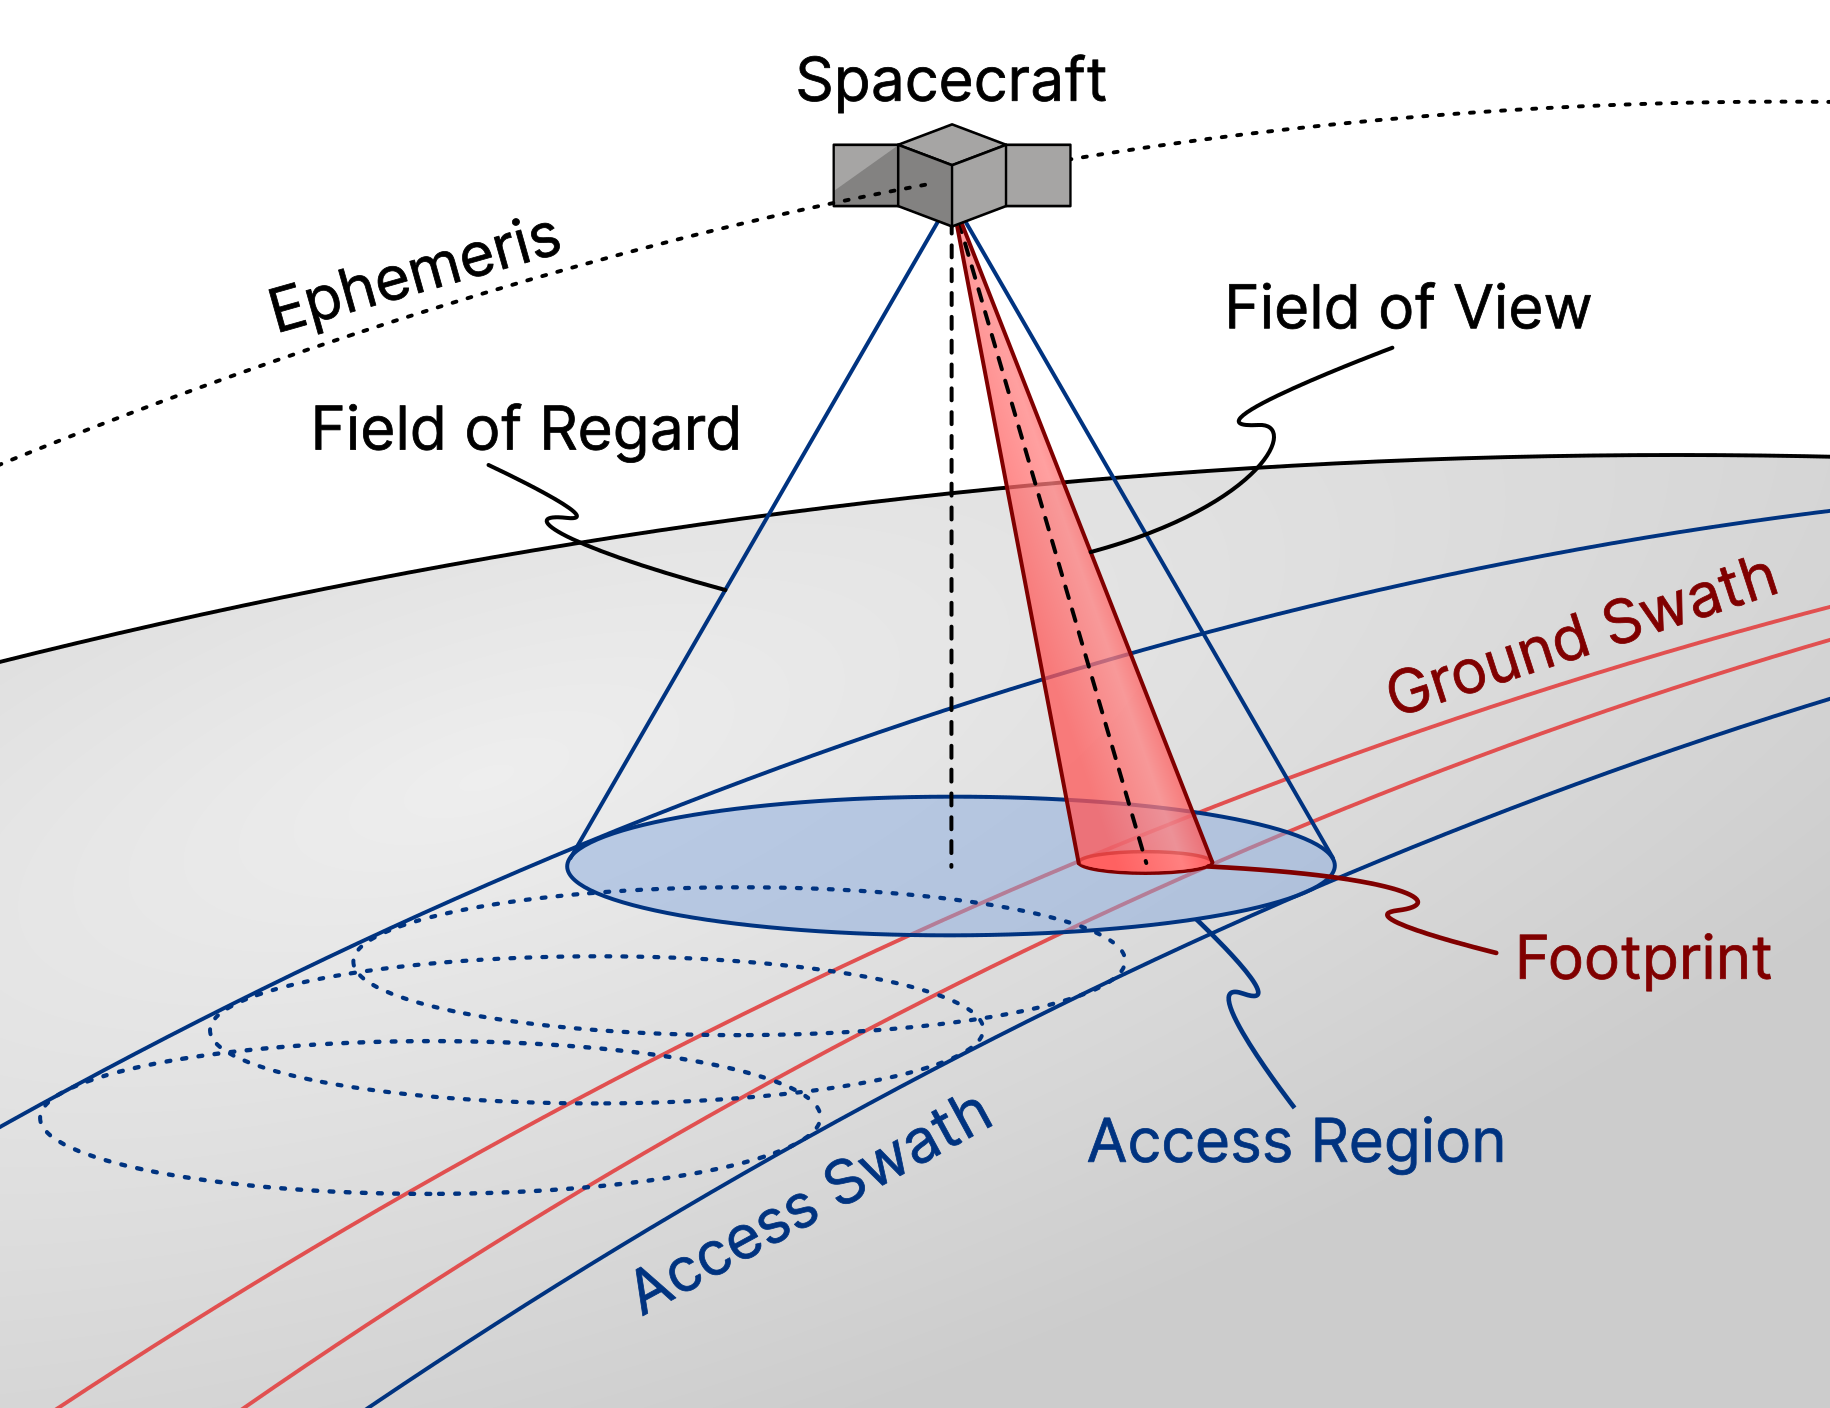
\includegraphics[width=\textwidth]{terminology.png} 
	\caption{General Illustration of Terminology}
	\label{fig:terminology} 
    \end{minipage}
    \hfill
    \begin{minipage}[c]{0.45\textwidth}
	\centering
	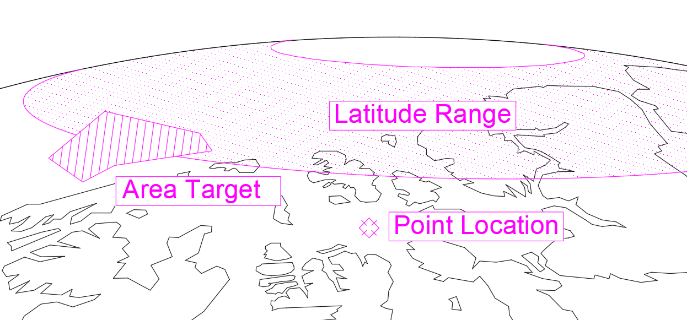
\includegraphics[width=\textwidth]{AOIs.png} 
	\caption{Different Types of Areas of Interest}
	\label{fig:AOIs} 
    \end{minipage} 
\end{figure}

%\begin{description} 
%
%    \item[Ephemeris] is a time series of orbital state vectors in a given
%	coordinate system. These state vectors have a position component,
%	$\sev{r}$, a velocity component, $\sev{v}$, and an epoch for each
%	vector, $e$. See section \ref{sgp4_section} for a more detailed
%	discussion on ephemerides.
%
%    \item[Area of Interest] An \gls{aoi} is a region on the Earth that is of
%	some particular importance to an operator. It is the region in which
%	one or more spacecraft should observe through some means. \glspl{aoi}
%	can be specified as a point location, an area target, or a latitude
%	range. Some examples of \glspl{aoi} are illustrated in \ref{fig:AOIs}.
%
%    \item[Field of View] The \gls{fov} is the extent to which a sensor or
%	instrument may observe the outside world at a given time. The size and
%	shape of an \gls{fov} varies based on the design of the sensor or
%	instrument. \glspl{fov} can theoretically describe any volume of space
%	but, for the purposes of this thesis, it may be assumed that they are
%	conical. Specifically, the \gls{fov} is defined by a single half-angle,
%	$\theta$. Suppose an instrument is pointing along some vector,
%	$\sev{u}$. Let us define another vector, $\sev{v}$ such that the angle
%	between it and $\sev{u}$ is $\theta$. The \gls{fov} is the volume
%	described by rotating $\sev{u}$ around $\sev{v}$.
%
%
%    \item[Field of Regard] The \gls{for} is similar to the \gls{fov} but
%	instead of being the area a sensor can observe in a single time
%	instant, the \gls{for} is the volume of space a sensor can possibly
%	observe by changing its orientation. Typically, it is constrained by
%	some physical or operational constraint. It is not possible to observe
%	the entire \gls{for}; Rather, only a subset of the \gls{for} can be
%	observed. This subset is the instrument's \gls{fov}.  For example, let
%	us consider an optical sensor fixed to a spacecraft orbiting the earth.
%	The position of the sensor at particular time instant is given by the
%	spacecraft's orbit and cannot be changed unless a propulsive manoeuvre
%	is performed.  Of course, the position of sensor can be changed
%	slightly by changing the attitude of the spacecraft, since the
%	instrument is most likely not located at the spacecraft's centre of
%	mass. But, this can be ignored since the distance the instrument can
%	translate is negligible compared to its orbit.  Conversely, The
%	orientation of the instrument can be changed, and this has a meaningful
%	effect on the \gls{for}. If no constraints are put on the attitude of
%	the spacecraft, the \gls{for} is everywhere, since the instrument can
%	be pointed in any direction. This is not always true though so let us
%	say the spacecraft can only point an angle, $\alpha$, off nadir.  The
%	\gls{for} would then be the cone described by the half-angle $\alpha +
%	\theta$, where $\theta$ is again the half-angle of the conical sensor.
%	Figure \ref{fig:fovfor} for an illustration of this example.  The
%	larger blue cone is the \gls{for}. The red cone is the sensor's actual
%	\gls{fov}. Its boresight is offset from the blue cone's.
%
%    \item[Footprint] The footprint is the area on Earth that can be observed by
%	an instrument's \gls{fov} or \gls{for} at a given time. It can be found
%	by intersecting the \gls{fov} or \gls{for} with the surface of the
%	Earth.  These intersection points form a boundary and the enclosed area
%	within this boundary is the footprint. For clarity, it should be
%	assumed that footprint refers to an \gls{for}'s footprint, unless
%	otherwise specified.
%
%    \item[Swath] If a sensor is moving over time, its footprint will move with
%	it. A swath is the union of all footprints over a time range.  It is
%	the region on Earth that can be possibly observed at some point by the
%	sensor.
%
%    \item[Horizon Swath] A horizon swath is a special case where the entire
%	Earth is within the sensor's \gls{for}. This may be true for certain
%	\gls{rf} payloads. In this case, the sensor can only `see' up until the
%	horizon. That is, the `horizon' footprint is all of the points on Earth
%	whose tangent line intersects with the sensor. Again, as the horizon
%	footprint moves, this forms the horizon swath.
%
%\end{description}



\section{Operations Scenario}

\gls{pops} is being developed to plan operations for missions at \gls{sfl} but,
to maintain the privacy of their customers' operations strategies, we shall
examine an imaginary scenario that is realistic but hypothetical. Given that
\gls{pops} is meant to be a general mission planning software, a hypothetical
mission scenario is still a valid example. Throughout this thesis, references
and examples will be made with this mission scenario in mind.

A common technique of remote sensing is Tip-and-Cue \cite{ali_tip_2021}.  In
this observation mode, multiple sensor systems are used to track both
stationary and moving targets over a wide area with high accuracy. First, a
sensor with a wide \gls{fov} is used to detect potential targets and these
targets are passed to another more accurate sensing system as ‘tips.’ The more
accurate system is then ‘cued’ to sense these potential targets. This is
especially useful for situations where the more accurate sensing system has a
limited \gls{fov}.

\begin{figure}[h]
    \centering
    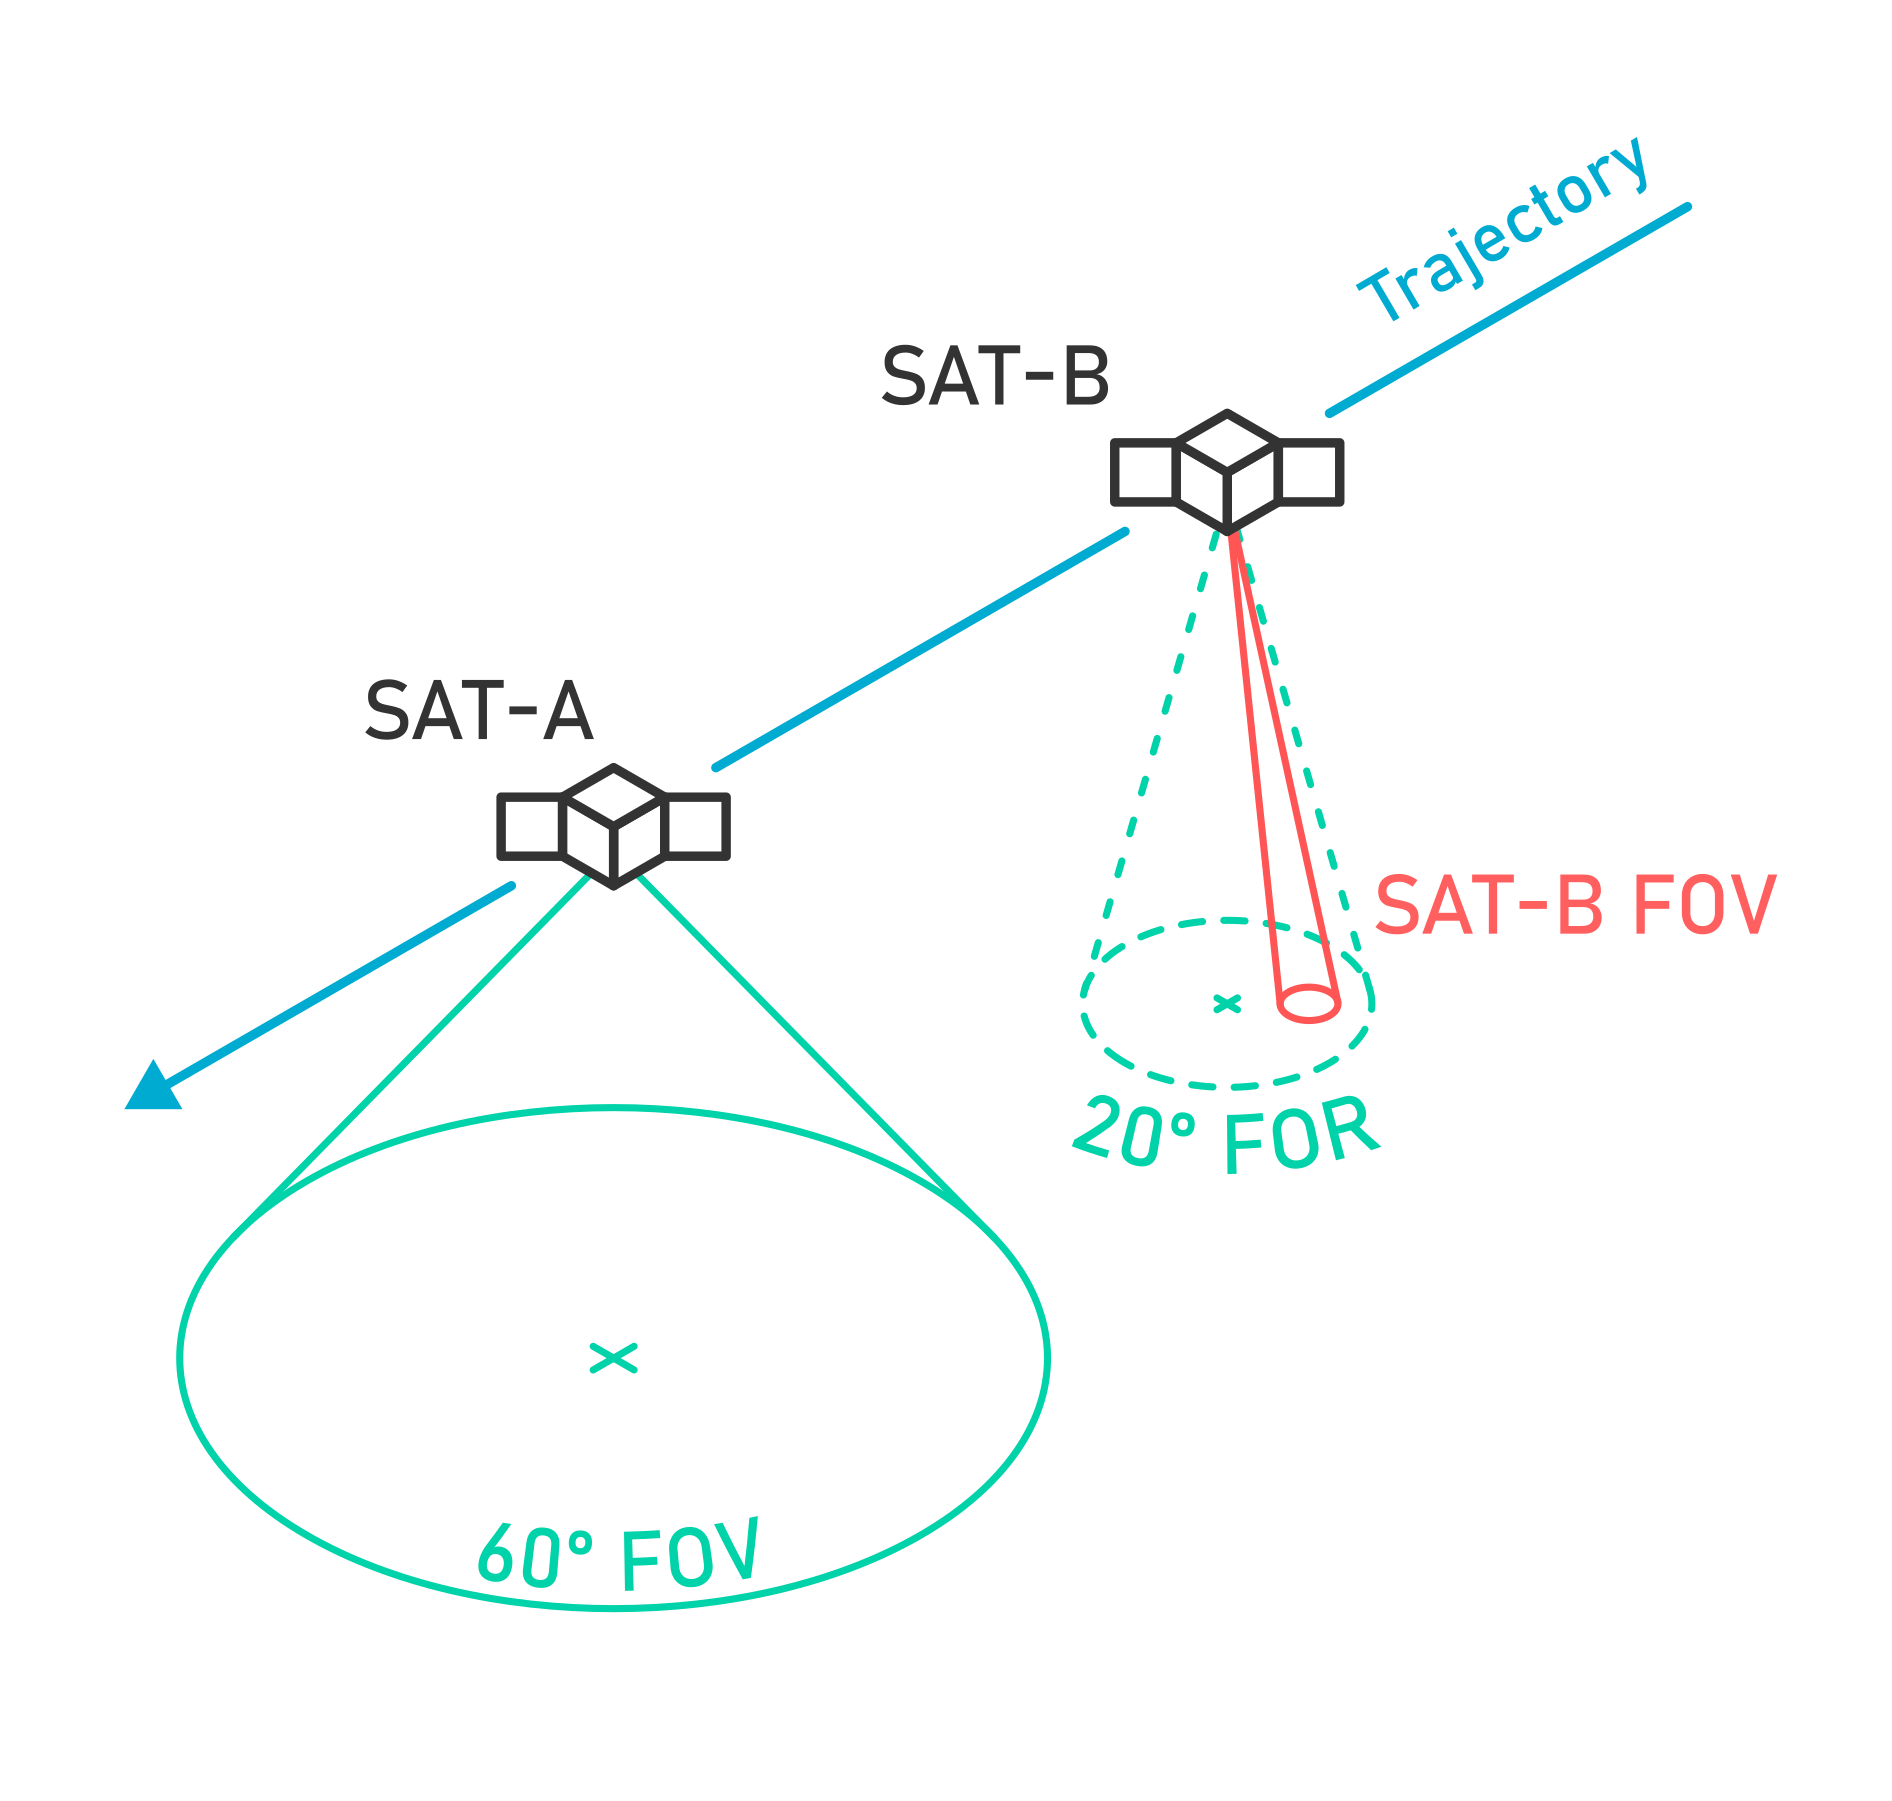
\includegraphics[width=0.6\textwidth]{EG-SAT.png} 
    \caption{EG-SAT Example Mission Scenario}
    \label{fig:eg-sat-1} 
\end{figure}

Let us say, as part of the “EG-SAT” mission, which is an imaginary mission, we
have a two-satellite constellation in formation where Sat-A leads Sat-B. Sat-A
has a course conical imager with a wide $60^\circ$ off-nadir \gls{fov} but low
ground resolution.  Sat-B has a fine conical imager with high ground resolution
but narrow \gls{fov}.  For the best coverage, Sat-A is always pointed at the
nadir.  Sat-B has some freedom and can be pointed $20^\circ$ off-nadir by
changing the spacecraft’s attitude.  It should be noted that since Sat-A’s
sensor is never pointed away from the nadir during payload operations, its
\gls{fov} is equivalent to its \gls{for}. Figure~\ref{fig:eg-sat-1} illustrates
the configuration of the EG-SAT mission.  The solid green lines under Sat-A
describe the $60^\circ$ \gls{fov} and footprint on the Earth. It's solid
because the \gls{fov} is equivalent to the \gls{for}. The dashed green lines
under Sat-B indicate the $20^\circ$ \gls{for} and access region. The red lines
indicate Sat-B's \gls{fov}. Notice how the \gls{fov} can be pointed in any
direction within the \gls{for}. This mission has two operations modes: 

\begin{figure} 
    \centering
    \begin{minipage}[c]{0.49\textwidth}
	\centering
	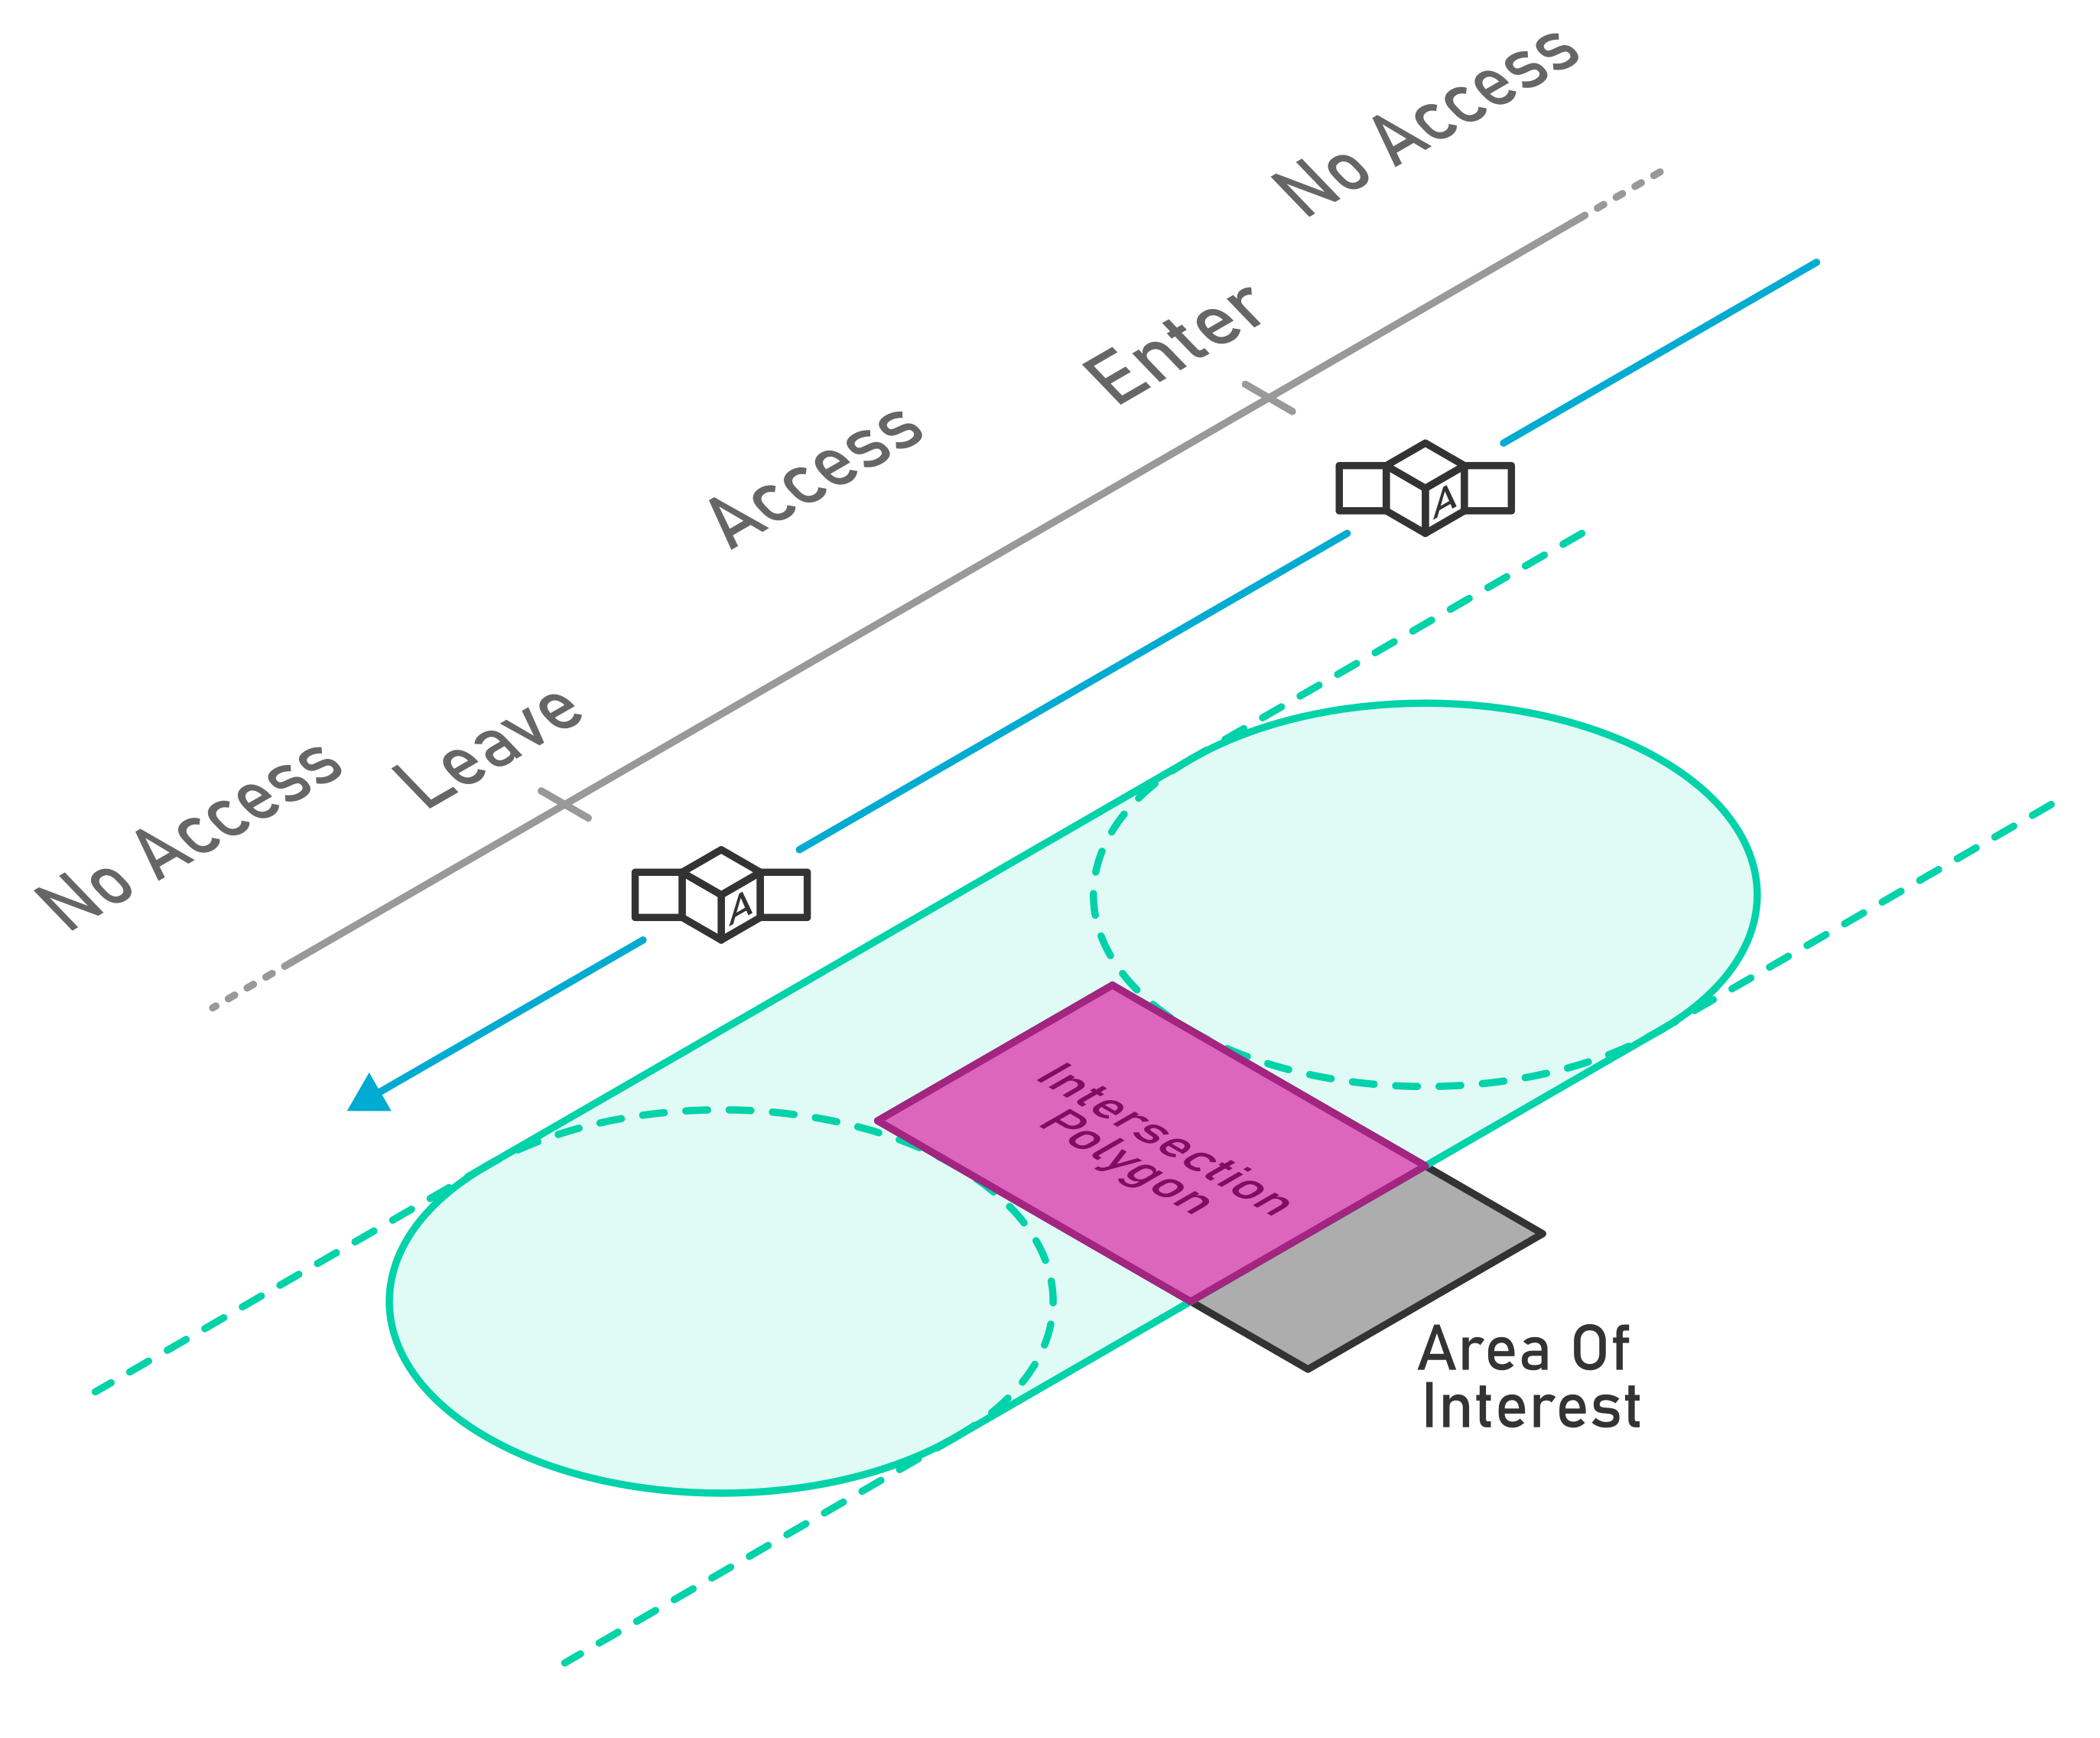
\includegraphics[width=\textwidth]{EG-SAT - obs 1.png} 
	\caption{Course Imaging}
	\label{fig:eg-sat-2} 
    \end{minipage}
    \hfill
    \begin{minipage}[c]{0.49\textwidth}
	\centering
	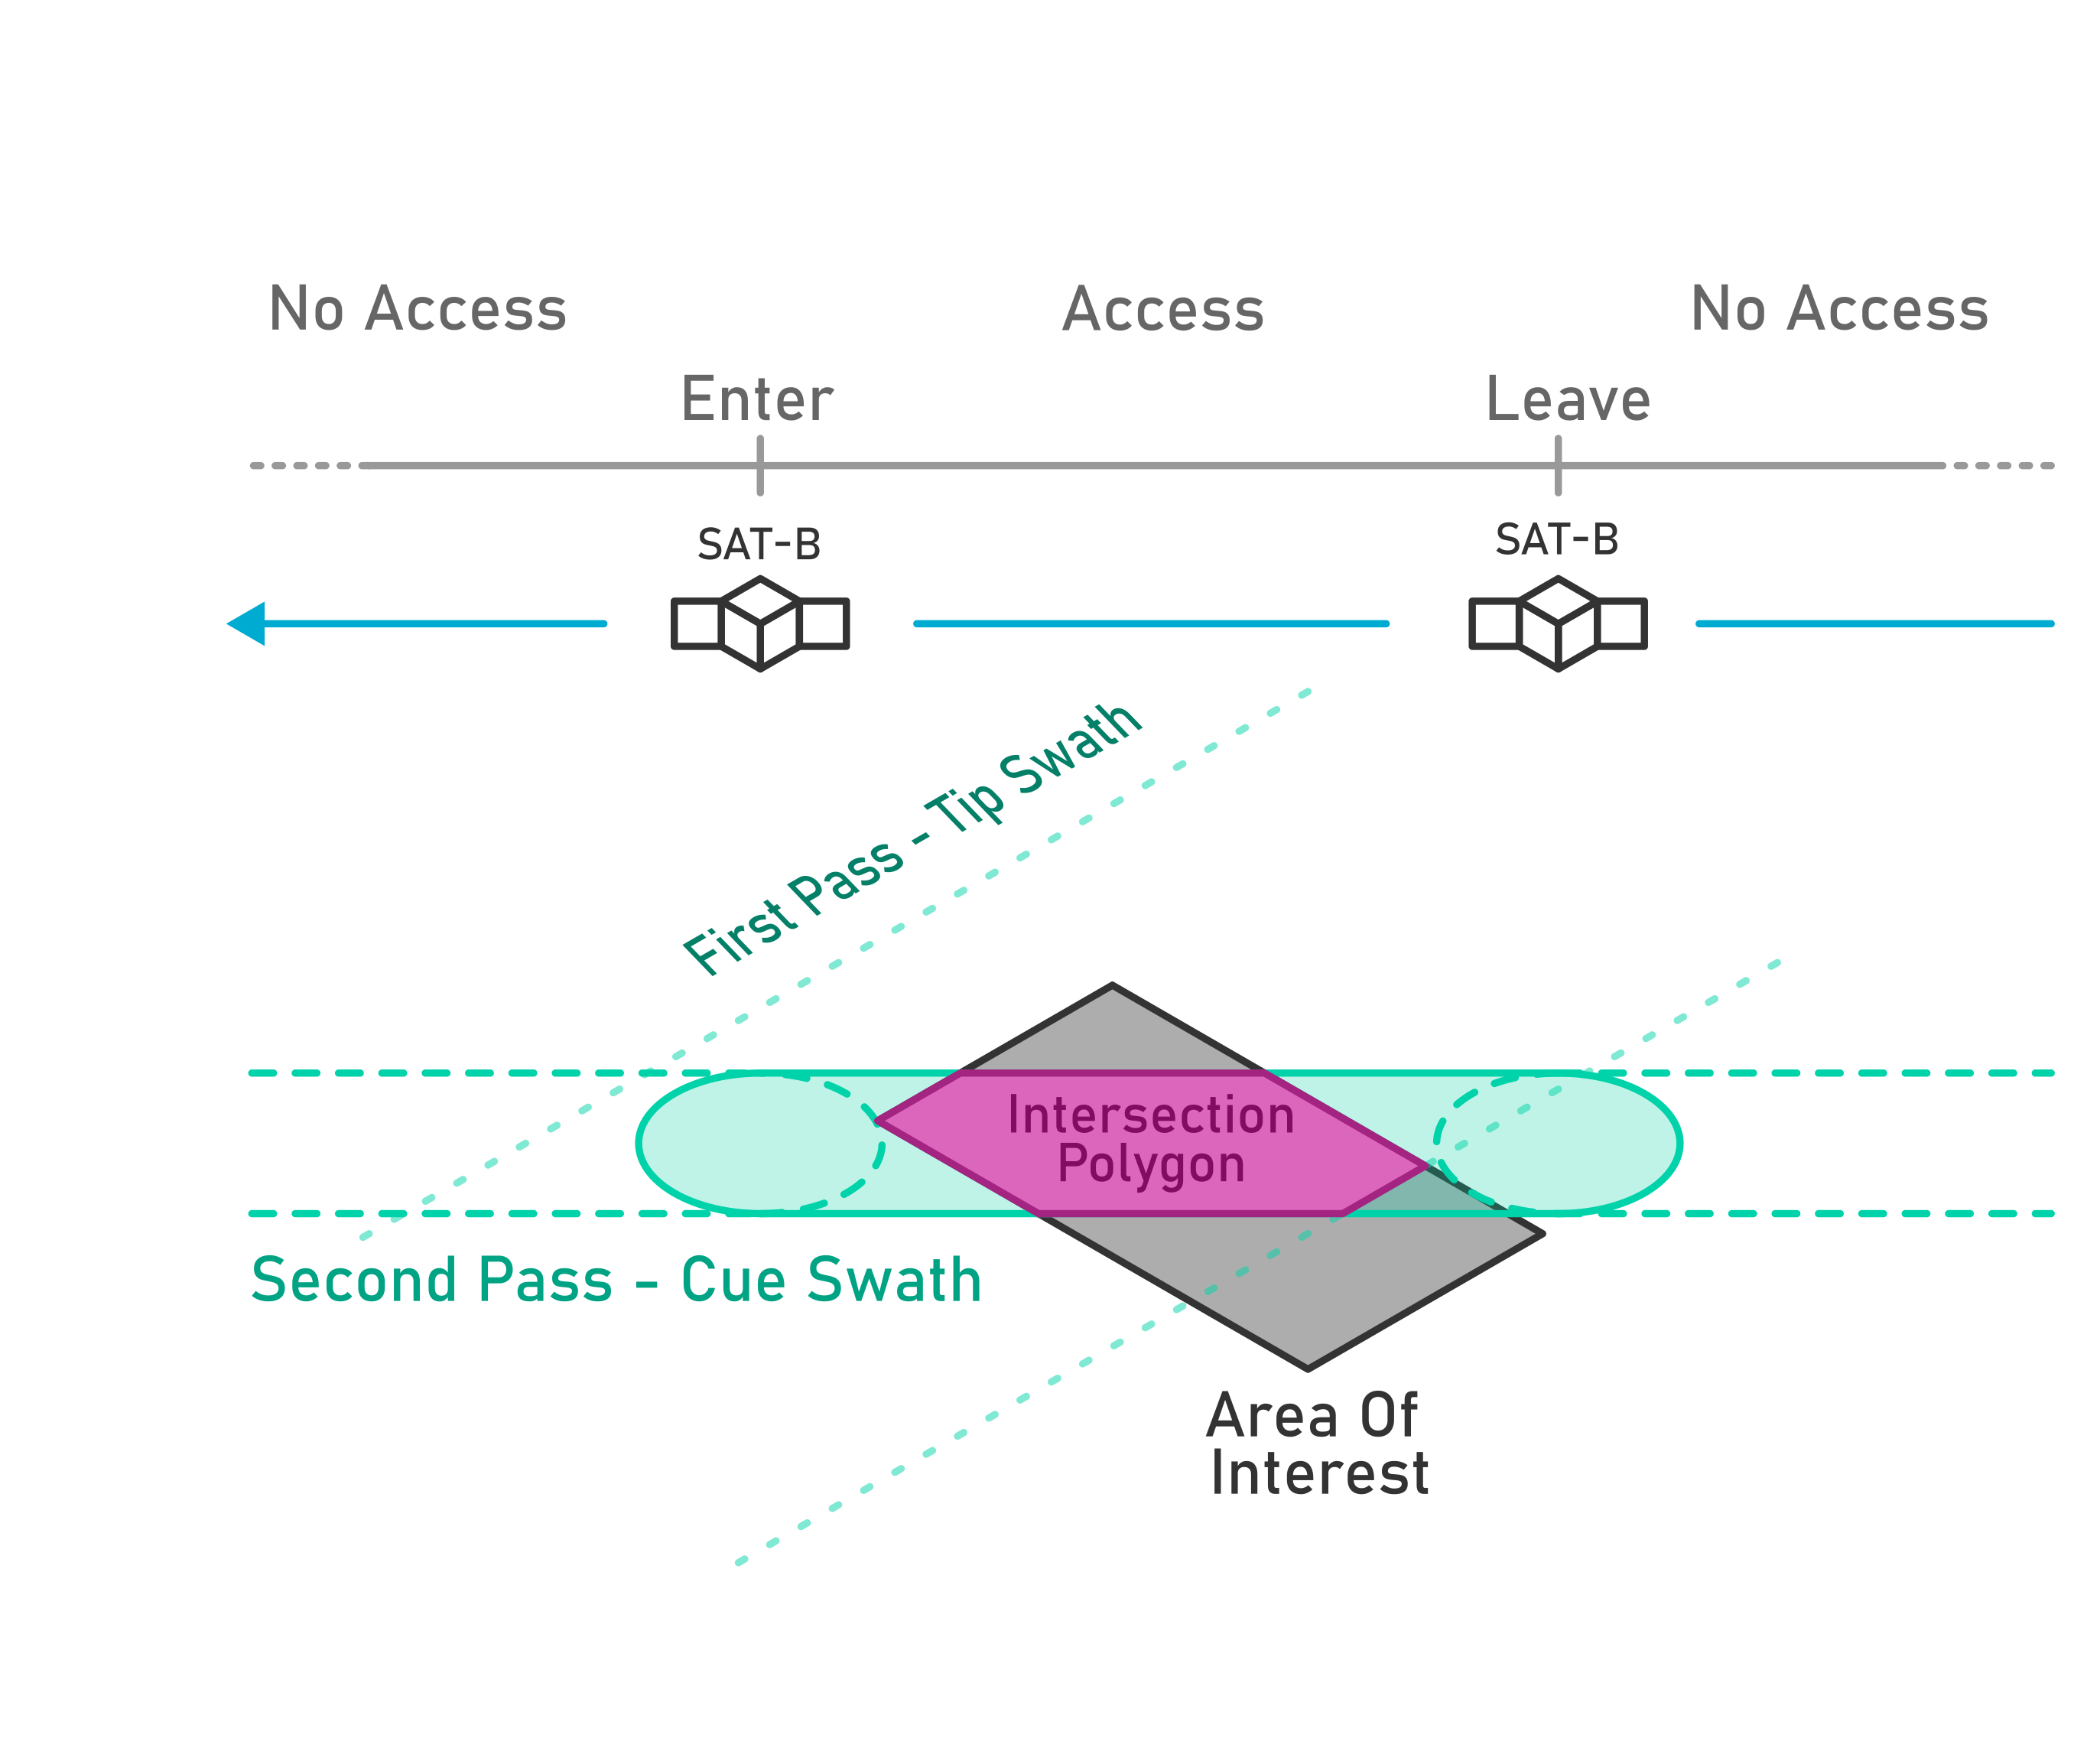
\includegraphics[width=\textwidth]{EG-SAT - obs 2.png} 
	\caption{Next-Pass Tip-and-Cue Imaging}
	\label{fig:eg-sat-3} 
    \end{minipage} 
\end{figure}

\begin{description} 

    \item[Course Imaging] In this mode, Sat-A must take images from all or part
	of an Area of Interest. This sensor data must then be recorded and
	downlinked at a ground station some time in the future.

    \item[Tip-and-Cue Imaging] Sat-A performs Coarse Imaging during the first
	pass over an Area of Interest. This data is then downlinked to a ground
	station which processes it and commands Sat-B to take fine images over
	the Area of Interest on the next pass.

\end{description}

The Course imaging mode is illustrated in Figure~\ref{fig:eg-sat-2}. When the
\gls{fov} of Sat-A first intersects the \gls{aoi}, Sat-A begins taking in
sensor data. This is represented by the solid green region.  When the \gls{fov}
no longer intersects the \gls{aoi}, Sat-A stops recording imagery data.
Typically for Area Target or Latitude Range \glspl{aoi} a satellite will not be
able to observe the entire area. As such, the region where the ground swath (or
access swath) intersects with the \gls{aoi} is called the Intersection Polygon
which is represented in magenta. 

The first pass of the Tip-and-Cue Imaging mode is equivalent to course imaging
and can still be seen in Figure~\ref{fig:eg-sat-2}. The next pass component
Tip-and-Cue Imaging mode is illustrated in Figure~\ref{fig:eg-sat-3}. It is
assumed that between the first and next pass a ground contact has occurred and
Sat-B has been given fine imaging targets. Since, we cannot know where
potential targets will be on the next pass a priori, we must rely on Sat-B's
\gls{for}.  This access region of Sat-B is represented by the green region. For
this mode, the intersection polygon is not with the entire \gls{aoi}, rather it
is the Intersection Polygon from the previous pass. This is the area that
intersects both the \gls{aoi}, first pass ground swath, and next pass access
swath.  


\section{Opportunity Filtering} \label{sec:opp-filtering}

Opportunity Filtering is the process of taking an infinite set of potential
observations and filtering out opportunities based on a set of constraints.
Opportunities, are instances or periods of time when a particular observation
mode can be performed on an \gls{aoi}. \gls{pops} is intended to be a
generalizable and easily expandable tool but the process of filtering for
observation opportunities is inherently specific to a mission’s operation’s
strategy.  For this reason, opportunity filtering functionality must be
developed individually for each operations mode.  Filtering, may be done by
stringing together primitive utilities and saving the result. 

The inputs to the opportunity filtering process are: satellite ephemerides and
an \gls{aoi}. An opportunity filter may need to consider multiple satellites,
hence multiple ephemerides. These ephemerides form the basic component from
which all other search data is calculated. It is from this search data that we
`filter' for opportunities. We must provide also an \gls{aoi}.  Without it, no
opportunities can be found as an opportunity cannot exist without an area to
observe.

Let us now introduce our primitive utilities. By primitive utilities, it is not
implied that they are in any way simple or trivial to implement but, rather,
they form the most basic operations and cannot be simplified to another, more
basic, form.  These primitive utilities are implemented by the \gls{atu}
service which is discussed in Section~\ref{sec:atu} but for now we will be
discussing them at a high level. For the EG-SAT mission, we will only need
three utilities.

The first primitive utility is the \textbf{Swath Utility}. From a satellite
Ephemeris and the swath half-angle, the Swath Utility calculates the
corresponding swath over that time range. The swath that is generated by this
utility not only contains the bounded region of the swath but also the
footprint or access region at each time instant. Note, it has not been
specified whether the generated swath is an access swath or ground swath.  The
process for calculating either is equivalent so a distinction is not made.  It
is up to the developer using the service to understand whether the outputted
swath is one or the other.

The second primitive utility is the \textbf{Polygon Intersection Utility}.
From a swath and a ground polygon, this utility calculates both the access
times and the intersection polygon between the swath and the input polygon. The
access times are timestamps which specify when a satellite `enters' or `leaves'
an access. The input polygon can be any polygon weather it is an \gls{aoi} or
it is derived through some other process.

The third primitive utility is the \textbf{Ground Access Utility}. This is a
sub-case of the Polygon Intersection Utility, where the ground polygon is just
a point. It behaves the same way where, given a swath and a point target, the
utility generates a list of access times (but not an intersection polygon since
a point cannot be sub-divided).

From these primitives, opportunity filtering will only output access times,
intersection polygons, or swaths. The concept of an `opportunity' is, to some
extent, completely arbitrary and not concretely defined. For \gls{pops}, an
opportunity may be represented through two components, \textit{when} and
\textit{where}. That is, what is the area that may be observed and when can one
or more spacecraft observe it. 

With a basic understanding of opportunity filtering, let us now walk through
defining filters for the two EG-SAT modes. For each filter, it is helpful to
define: the inputs, required constraints, and what constitutes an opportunity.

\subsection{Course Imaging Filter}

\begin{description} 

    \item[Inputs:]  Sat-A Ephemeris and \gls{aoi}

    \item[Constraints:] $60^\circ$ Ground Swath and an \gls{aoi}

    \item[Opportunity:] 1 Access Time (enter + leave) and 1 Intersection Polygon

\end{description} 

\begin{figure}[h]
    \centering
    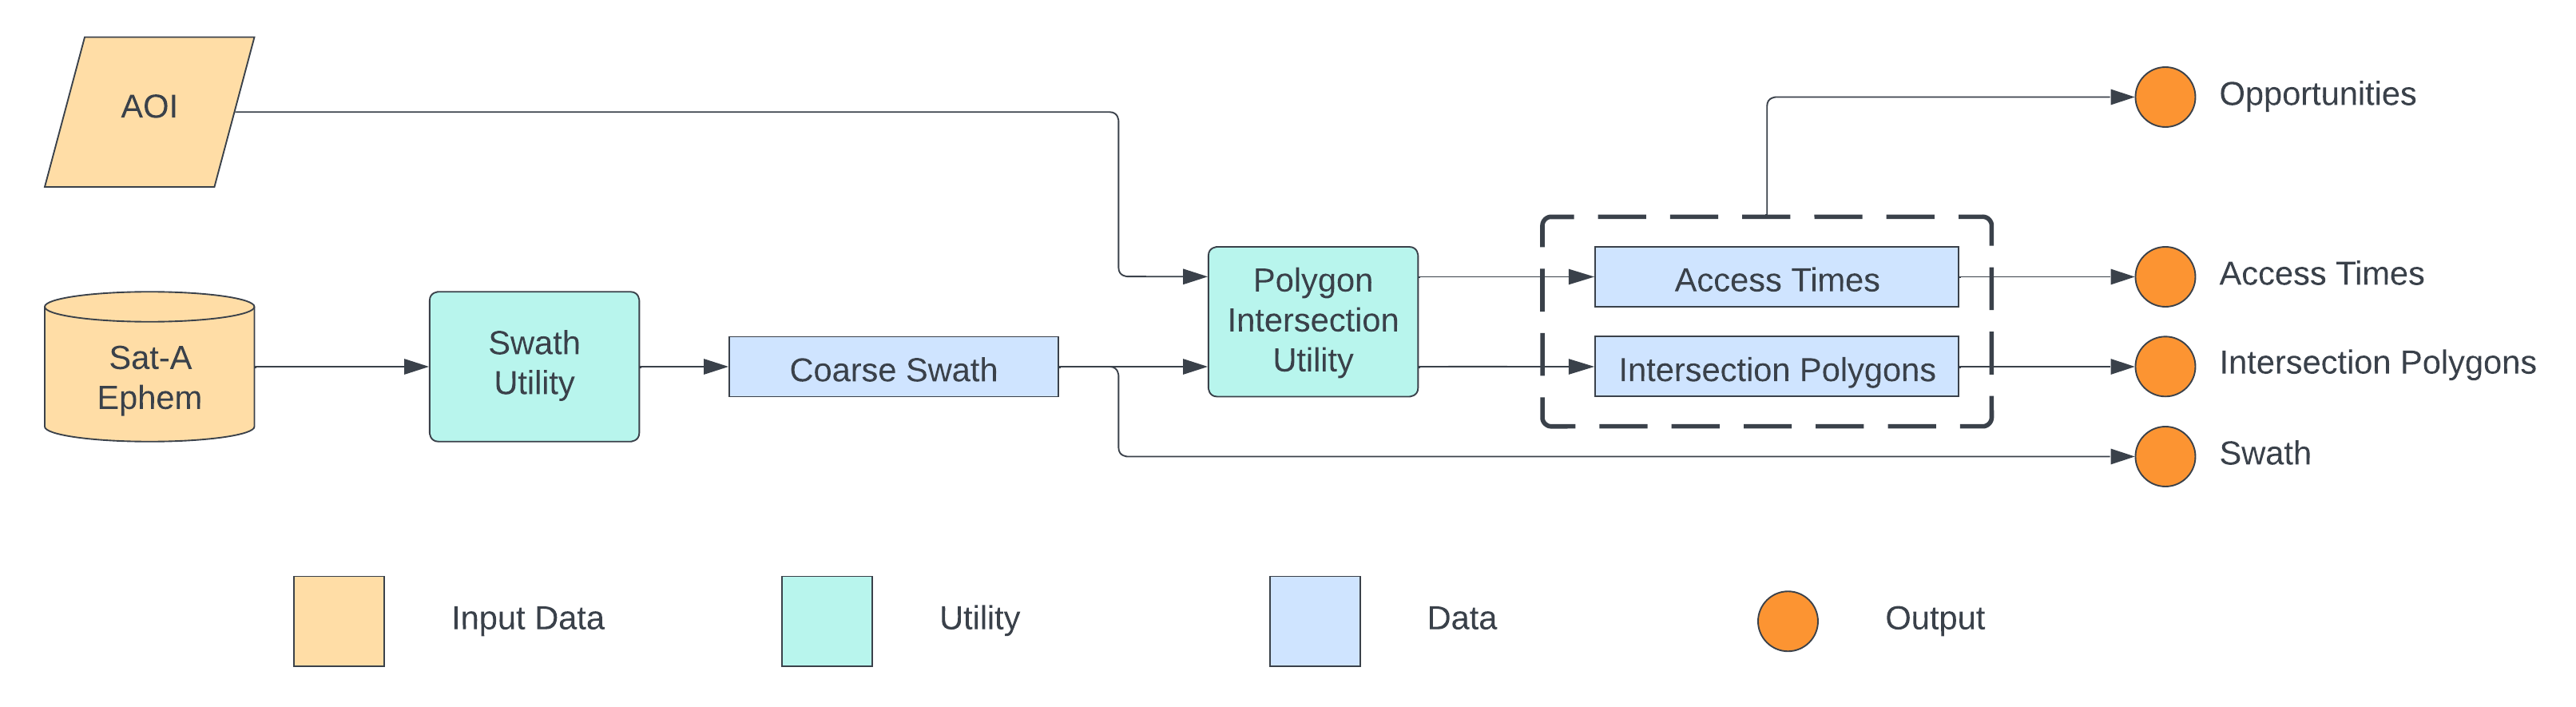
\includegraphics[width=\textwidth]{Coarse Imaging.png} 
    \caption{Coarse Imaging Filter}
    \label{fig:filter-1} 
\end{figure}

It is useful to display the filtering process graphically at a high level.
This can be seen in Figure~\ref{fig:filter-1}. First, from Sat-A's ephemeris,
it's coarse imaging swath is generated using the Swath Utility. Then, the swath
is intersected with the \gls{aoi} through the Polygon Intersection Utility. The
output of which generates some access times and intersection polygons. When
these are generated, they are each linked together as opportunities. The
outputs of the filter are firstly the opportunities, the access times,
intersection polygons, and swath data. All of this search data is recorded
since it may be referenced at a later point for displaying the results or for
further filtering.

\subsection{Tip-and-Cue Imaging Filter}

\begin{description} 

    \item[Inputs:]  Sat-A Ephemeris, Sat-B Ephemeris, and  \gls{aoi}

    \item[Constraints:] $60^\circ$ Ground Swath (tip), $20^\circ$ Access Swath (cue), and an \gls{aoi}

    \item[Opportunity:] 1 Tip Access Time, 1 Cue Access Time and 1 Intersection Polygon

\end{description} 

\begin{figure}[h]
    \centering
    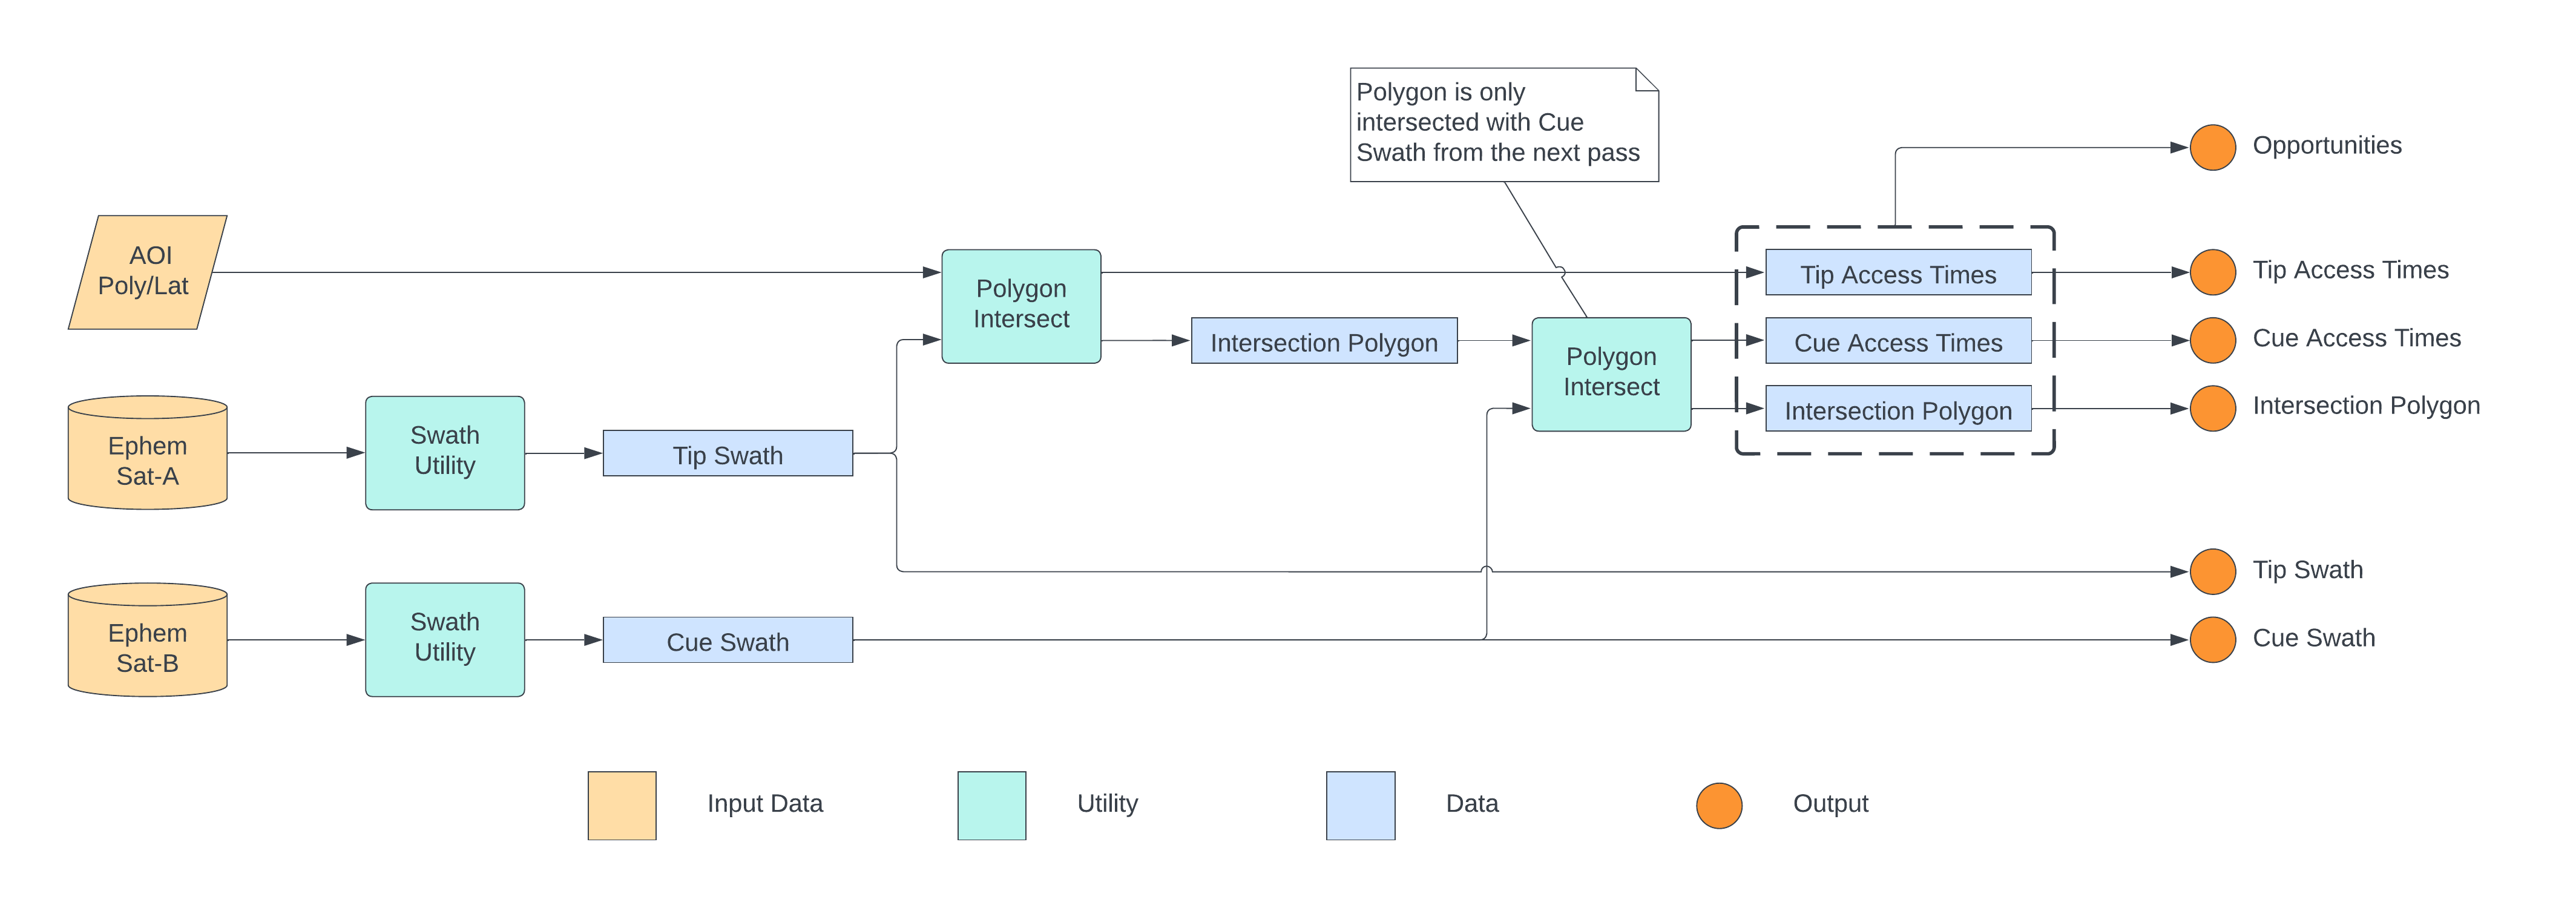
\includegraphics[width=\textwidth]{TNC Imaging.png} 
    \caption{Tip-and-Cue Imaging Filter}
    \label{fig:filter-2} 
\end{figure}


The Tip-and-Cue Imaging Mode can be seen in Figure~\ref{fig:filter-2}. The
first stage is the same as the Coarse Imaging filter. A tip swath, which is the
coarse imaging swath from Sat-A, is intersected with the \gls{aoi} to generate
access times and intersection polygons. In the second stage, Sat-B's ephemeris
is used to generate a cue swath, which is the fine imaging access swath. This
is then intersected with the intersection polygon from the previous stage. One
complexity that is hard to capture in the diagram is that the cue swath must be
subdivided into passes, such that the cue swath can be intersected on the next
pass. From the second Polygon Intersection Utility, Cue Access Times and final
intersection polygons are produced. These are linked together with the Tip
Access Times from the previous pass. All of this information is then outputted
along with the Tip and Cue Swaths.

This was a high-level overview of how Opportunity Filters are constructed. How
they are implemented and how the output data is used is discussed in the next
chapter.


\section{Orbit Propagation}

For \gls{pops} it is essential that there is some way of propagating a
satellite's orbit. That is, we must have a way of estimating a satellites
position at a given time. Very accurate methods of propagation do exist, but
these are involved and may be time consuming to implement. The desire for
\gls{pops} currently is to have \textit{some} method of propagation that is
suitably accurate rather than a very accurate method that would take a great
deal of time to develop.

\subsection{NORAD Two-Line Element Sets}

The United States Space Force tracks all detectable Earth \glspl{rso} and makes
this information public in the form of lists of \gls{norad} \gls{tle} sets.
\glspl{rso} are any natural or artificial object in Earth's orbit or any other
body.  This information is one of the only public sources of data regarding
Earth orbiting \glspl{rso}. Among these \glspl{rso} are \gls{sfl} spacecraft. A
\gls{tle} is a standard data format that contains a list of specialized orbital
elements at a specific time, referred to as the \gls{tle} epoch. \glspl{tle}
are inextricably linked to the `simplified perturbation models' family of
algorithms, specifically \gls{sgp4}.  Though less accurate than numerical
computation methods, these allow for quick and relatively accurate computation
of satellite trajectories.  This section is not intended to be an in-depth
reference of propagating satellite trajectories with \glspl{tle} but rather it
is a summary of the concepts as well as some of the literature.

Unfortunately, there have not been many publications made by the U.S. military
regarding the exact process to generate \glspl{tle}. This is essential because
the assumptions made in the creation of a \gls{tle} must be accounted for to
produce accurate propagation results. There are, though, a few publications of
note on this subject. Originally the source code for the `simplified
perturbation models' family of algorithms was defined explicitly in
\cite{hoots_spacetrack_1980}.  After some years, many purpose-built versions of
\gls{sgp4} were developed, each with their own assumptions and implementation
details. These were consolidated together in \cite{vallado_revisiting_2006},
which provided a number of tested implementations of \gls{sgp4} in a variety of
programming languages. Still today, this is the best reference for \gls{sgp4}.
Later, \cite{vallado_sgp4_2008} was published as a reference for generating
\glspl{tle} from ephemeris data. In addition, \cite{vallado_fundamentals_2001}
was published as an exhaustive reference on orbital dynamics which discusses at
length not only \glspl{tle} and \gls{sgp4} but also the underlying theory as
well as derivation examples.



\begin{figure}[h]
    \begin{verbatim}
    IDENTIFIER
    1 16609U 86017A   93352.53502934  .00007889  00000-0  10529-3 0  0342
    2 16609  51.6190 13.3340 0005770  102.5680 257.5950 15.59114070 44786
    \end{verbatim} 
    \caption{Example of a \gls{tle}}
    \label{fig:tle-ex} 
\end{figure}

An example of a \gls{tle} can be seen in Figure~\ref{fig:tle-ex} taken from
\cite{vallado_fundamentals_2001}.  As the name implies, there are two
69-character lines of data. Occasionally, a title is added for reference but
this is not required as part of the \gls{tle} definition. The data allocations
can be seen in Figure~\ref{fig:tle-legend}. The corresponding allocations for
each reference number can be seen in Table~\ref{tab:tle-line-1} and
Table~\ref{tab:tle-line-2} for lines 1 and 2 respectively.

\begin{figure}[h]
    \centering
    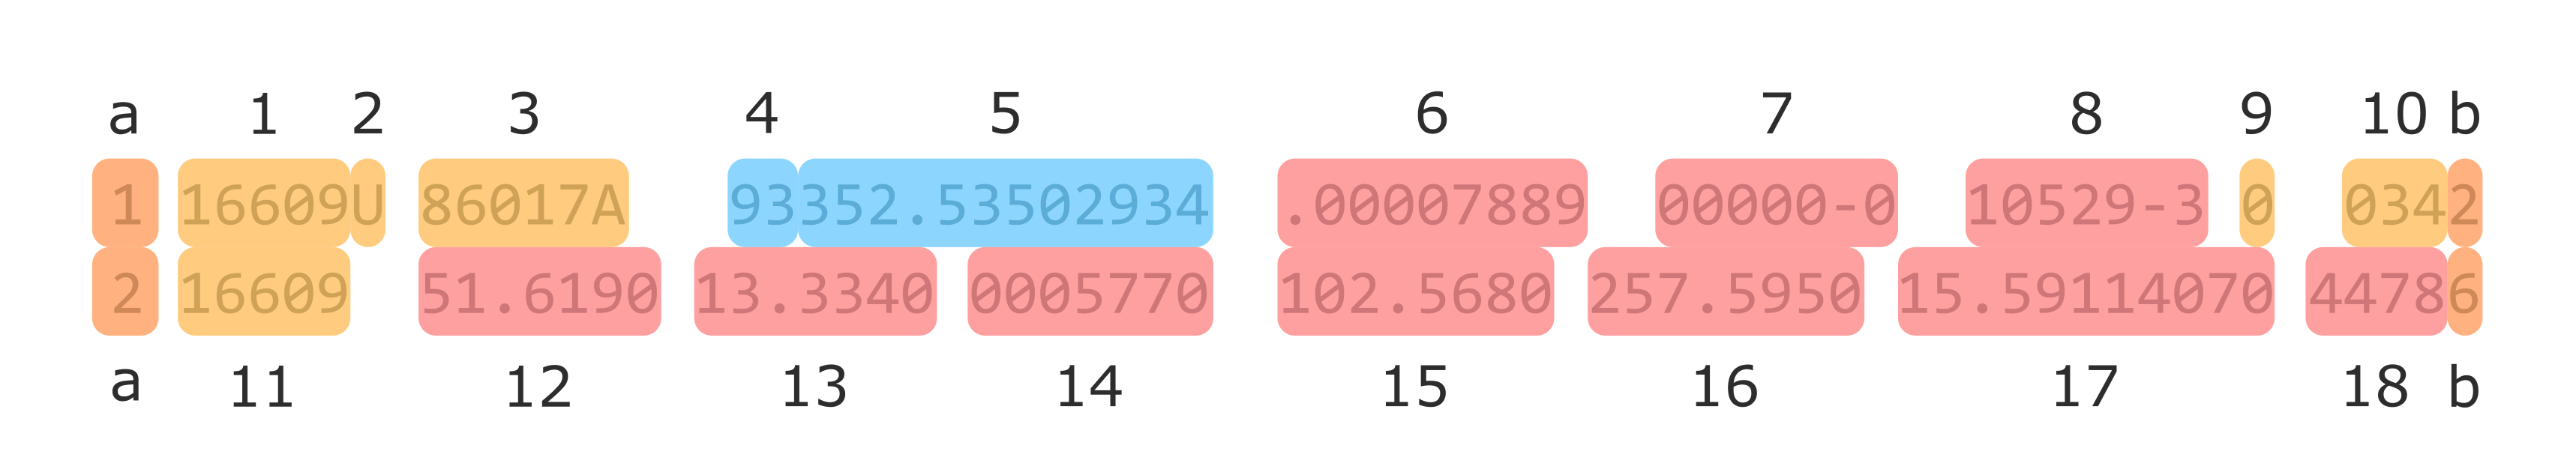
\includegraphics[width=\textwidth]{TLE.png} 
    \caption{TLE Data Format}
    \label{fig:tle-legend} 
\end{figure}

\begin{table}[!htb]\small
%\setlength{\tabcolsep}{6pt}

\begin{minipage}{.49\textwidth}
\centering

\caption{Data Format, Line 1}
\label{tab:tle-line-1}

\medskip

\begin{tabular}{|c|ll|}
\hline

\multicolumn{1}{|l|}{} & \multicolumn{1}{l|}{Description} & \multicolumn{1}{l|}{Units} \\ \hline
a  & Line Number   &   \\ \hline
1  & Satellite Number   &   \\
2  & Classification (U/C/S)   &   \\
3  & International Designator   &   \\
4  & \gls{tle} Epoch, Year   & years  \\ 
5  & \gls{tle} Epoch, Day   & days  \\
6  & Mean Motion, $1^{\mathrm{st}}$ Derivative & rev/day  \\
7  & Mean Motion, $2^{\mathrm{nd}}$ Derivative    & rev/day$^3$  \\
8  & B* (B Star)   & $R_{\mathrm{Earth}}^{-1}$  \\
9  &  Ephem Type (always 0)  &   \\
10  &  Element Number  &   \\ \hline
b  & Checksum   &  \\
\hline

\end{tabular}
\end{minipage}\hfill
\begin{minipage}{.49\textwidth}
\centering

\caption{Data Format, Line 2}
\label{tab:tle-line-2}

\medskip

\begin{tabular}{|c|ll|}
\hline

\multicolumn{1}{|l|}{} & \multicolumn{1}{l|}{Description} & \multicolumn{1}{l|}{Units} \\ \hline
a  & Line Number   &   \\ \hline
11 & Satellite Number   &   \\
12 & Inclination   & $^\circ$  \\
13 & Right Ascension   & $^\circ$  \\
14 & Eccentricity &   \\
15 & Perigee & $^\circ$  \\
16 & Mean Anomaly & $^\circ$ \\
17 & Mean Motion & rev/day \\
18 & Orbit Number &  \\ \hline
b  & Checksum   &  \\
\hline

\end{tabular}
\end{minipage}


\end{table}

It is not essential to have a complete understanding of every term in a
\gls{tle}. Generally, they are meant to be consumed by an algorithm and are not
human readable. Despite this, it is good to have a general understanding of the
terms.  Elements 1-3 and 11 give us information about the satellite the
\gls{tle} has been generated for. Elements 4 and 5 give us the \gls{tle} epoch.
Elements 12-17 give us the independent orbit elements that can be used to
describe a satellite's orbit. Elements 6-8 describe the effects of
perturbations on that orbit. Lastly, Elements a, b, 9, and 10 give us
meta-information about the \gls{tle} itself. Even though the orbital elements
of a satellite can be extracted from a \gls{tle} and can then be used as inputs
for another propagator, this would be a mis-step and would produce erroneous
results. 

\begin{quote}
[\glspl{tle}] are `mean' values obtained by removing
periodic variations in a particular way. In order to obtain good predictions,
these periodic variations must be reconstructed (by the prediction model) in
exactly the same way they were removed by \gls{norad}. Hence, inputting
[\glspl{tle}] into a different model (even though the model may be more accurate or even
a numerical integrator) will result in degraded predictions. \cite{hoots_spacetrack_1980}
\end{quote}


\subsection{Propagator}

Within the simplified general perturbations family of algorithms there are 5
orbital propagation models: SGP, SGP4, SDP4, SGP8, and SDP8. These are
analytical methods of approximating orbital state vectors at corresponding
epochs. SGP (Simplified General Perturbations) was originally developed in 1966
for near-Earth satellites (orbital periods less than 225 minutes). It was then
replaced by SGP4 and SDP4.  SGP4 was originally developed in 1970 for near
Earth Satellites and SDP4 was an extension for `deep-space' satellites (orbital
periods greater than 225 minutes) in 1979.  The SGP8/SDP8 models were developed
in 1980 to address deficiencies in the previous versions but ultimately, they
did not become widely used.  Today SGP4/SDP4 are the dominant models.  Since
there is a clear distinction between when SGP4 and SDP4 should be used, they
are collectively referred to as just `SGP4'. Since the original report
\cite{hoots_spacetrack_1980}, changes have not been made to the theory but
rather the code implementations.  It should be noted that \glspl{tle} are
accurate to around a kilometer at epoch and degrade rapidly
\cite{vallado_revisiting_2006}. The actual error of an individual \gls{tle}
varies on a case by case basis. One source of error is that maneuvers cannot be
taken into account when generating \glspl{tle}. So, if some thrusting is done
by a spacecraft to maintain a formation for example, \glspl{tle} generated
before the maneuver will not be accurate after the thrust has occurred. After
this thrust, new \glspl{tle} will need to be generated. 



\subsection{Coordinate Systems}

When using Earth-centric coordinate systems, there are generally two types:
\gls{eci} and \gls{ecef}. These are not reference frames themselves but only
refer to families or reference frames. They vary based on the exact definitions
for each axis.  \gls{eci} frames do move with the Earth's rotation; they
remain, as the name implies, inertially fixed and their axis are defined with
respect to celestial bodies. \gls{ecef} frames do move with the Earth's
rotation. As such, they are useful for Earth-sensing satellite operations since
coordinates in an \gls{ecef} frame can be directly converted into
Latitude-Longitude-Altitude coordinates, whereas with an \gls{eci} frame this
process is much more involved. The outputs of the \gls{sgp4} propagator, are in
the \gls{teme} coordinate reference frame which is an \gls{eci} reference
frame. \gls{teme} is not particularly useful and must be transformed. This
process is discussed later.



\section{Time Tag Commands}

At the \gls{sfl}, satellites are commanded through the use of the \gls{nsp}
\cite{kekez_nanosatellite_2010}.  \gls{nsp} commands are a custom standard
developed by \gls{sfl} to facilitate ground and intra-satellite communication.
They are designed to minimize the effects of low-bandwidth radio communication
links that are prone to error.  These commands handle all aspects of nominal
operation, from turning individual units on or off, to specifying attitude
modes or initiating data transfers.  Once a command is sent, it is executed
immediately upon being received. This raises the concern of how can a
spacecraft be commanded when it does not have a direct communication link with
a ground station. To address this, there exist \glspl{ttc}.  \glspl{ttc} are
\gls{nsp} commands that have been prepended with a timestamp and a group ID.
When the spacecraft’s system clock reaches the time specified in the timestamp,
that command is executed.  The group ID allows operators to group \glspl{ttc}
such that they may be considered as a collection rather than as separate
commands, allowing for reference or removal as a single unit.  \glspl{ttc} are
prepared in advance by an operator and uploaded in bulk to the spacecraft.
This allows operators to control the spacecraft when direct communication
cannot be established.



